\lab{Solitons}{Solitons}
\label{lab:solitons}

\objective{
We study traveling wave solutions of the Korteweg-de Vries (KdV) equation, using a pseudospectral discretization in space and a Runge-Kutta integration scheme in time.  }


Here we consider soliton solutions of the Korteweg-de Vries (KdV) equation. This equation is given by 
\[  \frac{\partial u }{\partial t} + u \frac{\partial u}{\partial x} + \frac{\partial^3 u}{\partial x^3} = 0.
\]
The KdV equation is a canonical equation that describes shallow water waves. 

The KdV equation possesses traveling wave solutions called solitons.  
These traveling waves have the form 
\[ u(x,t) = 3s \sech^2\left(\frac{\sqrt{s}}{2}(x - st - a)\right),
\]
where $s$ is the speed of the wave. 
Solitons were first studied by John Scott Russell in 1834, in the Union Canal in Scotland. 
When a canal boat suddenly stopped, the water piled up in front of the boat continued moving down the canal in the shape of a pulse.  

Note that there is a soliton solution for each wave speed $s$, and that the amplitude of the soliton depends on the speed of the wave. 
Solitons are traveling waves in the shape of a pulse, they are nonlinearly stable (bumped waves return to their previous shape), and they maintain their energy as they travel. 
They also enjoy an additional stability property: They play well with others. 
Two interacting solitons will maintain their shape after crossing paths. 


\section*{Numerical solution}
Consider the KdV equation on $[-\pi,\pi]$, together with an appropriate initial condition: 
\begin{align*}
	 &{ }u_t = -\left(\frac{u^2}{2} \right)_x - u_{xxx},\\
     &{ }u(x,0) = u_0(x).
\end{align*}
We will use initial data that is zero at the endpoints. This will allow us to use a pseudospectral method for periodic initial data to find a numerical approximation for the solution $u(x,t)$. 

If we use $N$ subintervals in space, we then obtain the spatial step $h = 2\pi/N$ and the grid points $\{x_j\}_{j=1} = \{-\pi,-\pi + h,\ldots,\pi-h\}$.  
Let $\mathcal{F}(u)(t) = \hat{u}(t)$ denote the Fourier transform of $u(x,t)$ (in space), so that 
\[
\mathcal{F}(u) = \hat{u}(k,t), \quad k=-N/2+1, \ldots, N/2.
\]
Similarly we let $\mathcal{F}^{-1}$ represent the discrete inverse Fourier transform.
Recall that $k$ represents the wave numbers in Fourier space; our code defines it by 
\begin{lstlisting}
# Dependencies for this lab's code:
from __future__ import division
from math import sqrt, pi
import numpy as np					
from scipy.fftpack import fft, ifft		
from mpl_toolkits.mplot3d.axes3d import Axes3D
import matplotlib.pyplot as plt
from matplotlib import cm

# Array of wave numbers.  This array is reordered in Python to 
# accomodate the ordering inside the fft function in scipy.
k = np.concatenate(( np.arange(0,N/2) ,
					 np.array([0])	,
					 np.arange(-N/2+1,0,1)	)).reshape(N,)
\end{lstlisting}


We now apply the Fourier transform to the KdV equation. In Fourier space, we obtain 
\begin{align*}
	\mathcal{F}(u)_t &= -\frac{ik}{2}\mathcal{F}(u^2)- (ik)^3\mathcal{F}(u).
\end{align*}
Let $U(t)$ be the vector valued function given by $U(t) = (u(x_j,t))_{j=1}^N$.
Let $\mathcal{F}(U)(t)$ denote the discrete Fourier transform of $u(x,t)$ (in space), so that 
\[
\mathcal{F}(U)(t) = (\mathcal{F}(u)(k,t))_{k=-N/2+1}^{N/2}.
\]
Similarly we let $\mathcal{F}^{-1}$ represent the discrete inverse Fourier transform.
Using the pseudospectral approximation in space leads to the system of ODEs
\begin{align}
	\mathcal{F}(U)_t =  -\frac{i}{2} \vec{k}\mathcal{F}\left( \mathcal{F}^{-1}(\mathcal{F}(U))^2\right) + i\vec{k}^3\mathcal{F}(U)
\end{align}
where $\vec{k}$ is a vector, and multiplication is done element-wise. In terms of $Y = \mathcal{F}(U)$, this simplifies to 
\begin{align}
	Y_t =  -\frac{i}{2} \vec{k}\mathcal{F}\left( \mathcal{F}^{-1}(Y)^2\right) + i\vec{k}^3Y
	\label{lab:solitons:pseudospectral}
\end{align}
and is implemented below.
\begin{lstlisting}
# Defines the left hand side of the ODE y' = G(t,y)
# defined above.
ik3 = 1j*k**3.
def G_unscaled(t,y):
	out = -.5*1j*k*fft(ifft(y,axis=0)**2.,axis=0)  + ik3*y        
	return out
\end{lstlisting}

Equation \eqref{lab:solitons:pseudospectral} is solved below, using a soliton as initial data for the KdV equation. 
Note that the Fourier transform must be applied to the soliton before solving, and that the final numerical solution must be transformed back from Fourier space before plotting. 
\begin{lstlisting}
N = 256
x = (2.*np.pi/N)*np.arange(-N/2,N/2).reshape(N,1)   # Space discretization
s, shift = 25.**2., 2.  							# Initial data is a soliton
y0 = (3.*s*np.cosh(.5*(sqrt(s)*(x+shift)))**(-2.)).reshape(N,) 

# Solves the ODE.
max_t = 
dt = # constant*N**(-2.)
max_tsteps = int(round(max_t/dt))
y0 = fft(y0,axis=0)
T,Y = RK4(G_unscaled, y0, t0=0, t1=max_t, n=max_tsteps)

# Using the variable stride, we step through the data, 
# applying the inverse fourier transform to obtain u.
# These values will be plotted.
stride = int(np.floor((max_t/25.)/dt))
uvalues, tvalues = np.real(ifft(y0,axis=0)).reshape(N,1), np.array(0.).reshape(1,1)
for n in range(1,max_tsteps+1):
	if np.mod(n,stride) == 0:
		t = n*dt
		u = np.real( ifft(Y[n], axis=0) ).reshape(N,1)
		uvalues = np.concatenate((uvalues,np.nan_to_num(u)),axis=1)
		tvalues = np.concatenate((tvalues,np.array(t).reshape(1,1)),axis=1)

fig = plt.figure()
ax = fig.gca(projection='3d')
ax.view_init(elev=45., azim=150)
tv, xv = np.meshgrid(tvalues,x,indexing='ij')
surf = ax.plot_surface(tv,xv, uvalues.T, rstride=1, cstride=1, cmap=cm.coolwarm,
						linewidth=0, antialiased=False)
tvalues = tvalues[0]; ax.set_xlim(tvalues[0], tvalues[-1])
ax.set_ylim(-pi, pi); ax.invert_yaxis()
ax.set_zlim(0., 4000.)
ax.set_xlabel('T'); ax.set_ylabel('X'); ax.set_zlabel('Z')
plt.show()
\end{lstlisting}

The method we have used requires the use of an algorithm for (ODE) initial value problems, such as the RK4 algorithm. The RK4 method is implemented below.
\begin{lstlisting}
def initialize_all(y0, t0, t1, n):
	""" An initialization routine for the different ODE solving
	methods in the lab. This initializes Y, T, and h. """
	
	if isinstance(y0, np.ndarray):
		Y = np.empty((n, y0.size),dtype=complex).squeeze()
	else:
		Y = np.empty(n,dtype=complex)
	Y[0] = y0
	T = np.linspace(t0, t1, n)
	h = float(t1 - t0) / (n - 1)
	return Y, T, h


def RK4(f, y0, t0, t1, n):
	""" Use the RK4 method to compute an approximate solution
	to the ODE y' = f(t, y) at n equispaced parameter values from t0 to t
	with initial conditions y(t0) = y0.
	
	'y0' is assumed to be either a constant or a one-dimensional numpy array.
	't0' and 't1' are assumed to be constants.
	'f' is assumed to accept two arguments.
	The first is a constant giving the current value of t.
	The second is a one-dimensional numpy array of the same size as y.
	
	This function returns an array Y of shape (n,) if
	y is a constant or an array of size 1.
	It returns an array of shape (n, y.size) otherwise.
	In either case, Y[i] is the approximate value of y at
	the i'th value of np.linspace(t0, t, n).
	"""
	Y, T, h = initialize_all(y0, t0, t1, n)
	for i in xrange(1, n):
		K1 = f(T[i-1], Y[i-1])
		tplus = (T[i] + T[i-1]) * .5
		K2 = f(tplus, Y[i-1] + .5 * h * K1)
		K3 = f(tplus, Y[i-1] + .5 * h * K2)
		K4 = f(T[i], Y[i-1] + h * K3)
		Y[i] = Y[i-1] + (h / 6.) * (K1 + 2 * K2 + 2 * K3 + K4)
	return T, Y
\end{lstlisting}

% 
% \begin{lstlisting}
% 
% \end{lstlisting}
% \begin{lstlisting}
% 
% \end{lstlisting}
% \begin{lstlisting}
% 
% \end{lstlisting}
\begin{figure}
\centering
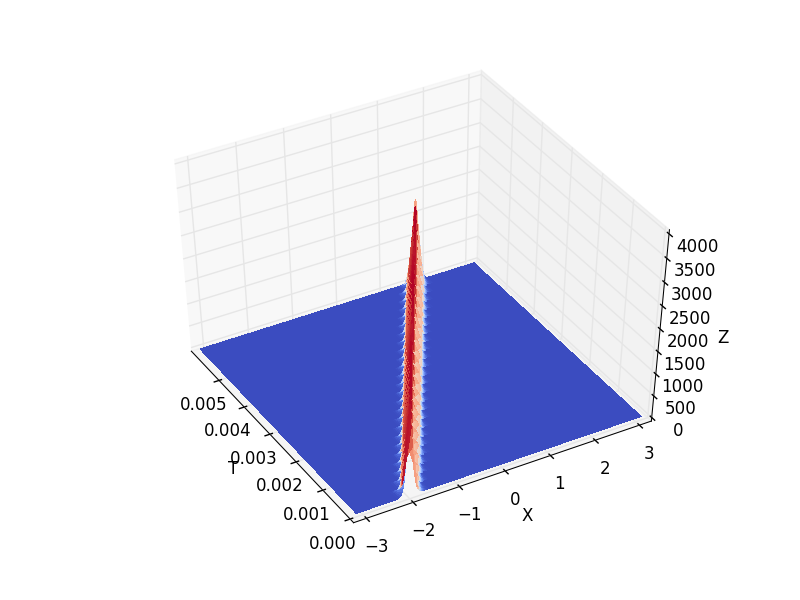
\includegraphics[width=\textwidth]{soliton.png}
\caption{The solution to Problem \ref{problem:solitons:single}.}
\label{fig:solitons:single}
\end{figure}


\begin{problem}
Run the code above to numerically solve the KdV equation on $[-\pi,\pi]$ with initial conditions 
\[
u(x,t=0) = 3s\sech^2\left(\frac{\sqrt{s}}{2}(x+a)\right),
\]
where $s = 25^2,$ $a = 2$. Solve on the time domain $[0,.0075]$. Define the stepsize variable {\tt dt} in the code above so that the method is numerically stable.  How small must {\tt dt} be? 

The solution is shown in Figure \ref{fig:solitons:single}.
\label{problem:solitons:single}
\end{problem}


\begin{figure}
\centering
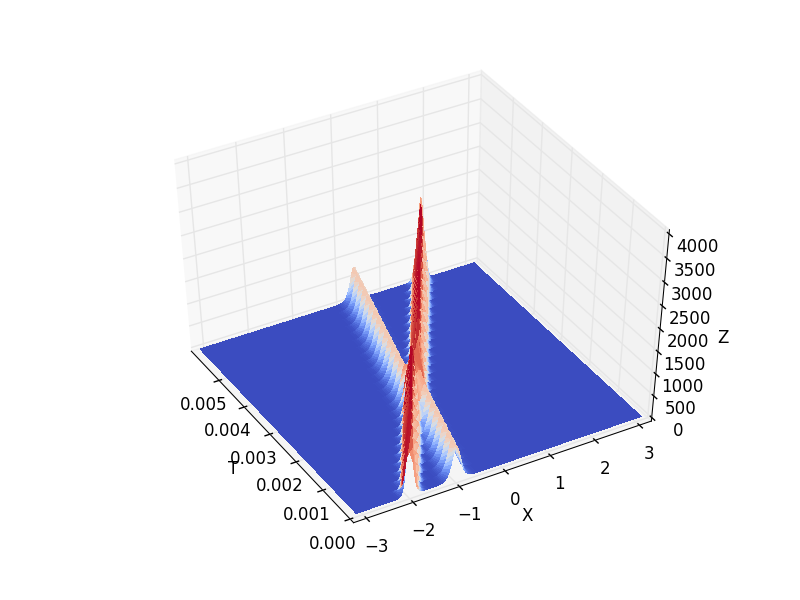
\includegraphics[width=\textwidth]{interacting_solitons.png}
\caption{The solution to Problem \ref{problem:solitons:interacting}.}
\label{fig:solitons:interacting}
\end{figure}


\begin{problem}
Numerically solve the KdV equation on $[-\pi,\pi]$. This time we define the initial condition 
to be the superposition of two solitons,
\[
u(x,t=0) = 3s_1\sech^2\left(\frac{\sqrt{s_1}}{2}(x+a_1)\right) + 3s_2\sech^2\left(\frac{\sqrt{s_2}}{2}(x+a_2)\right),
\]
where $s_1 = 25^2,$ $a_1 = 2$, and $s_2 = 16^2,$ $a_1 = 1$.\footnote{This problem is solved in \textit{Spectral Methods in MATLAB}, by Trefethen.} Solve on the time domain $[0,.0075]$.  How small must {\tt dt} be so that the method is numerically stable?  The solution is shown in Figure \ref{fig:solitons:interacting}.
\label{problem:solitons:interacting}
\end{problem}







\begin{problem}
	Consider again equation \eqref{lab:solitons:pseudospectral}. The linear term in this equation is 
	$i\vec{k}^3Y$. This term contributes much of the exponential growth in the ODE, and responsible for 
	how short the time step must be to ensure numerical stability. Make the substitution $Z = e^{-ik^3t}Y$ and find a similar ODE for $Z$. This essentially allows the exponential growth to be scaled out (it's solved for analytically). Use the resulting equation to solve the previous problem. How short can the time step be made? 
\end{problem}











% 
% The discrete Fourier transform (DFT) of $f$, denoted by $\hat{f}$ or $\mathcal{F}(f)$, is given by
% \[
% \hat{f}(k) = h \sum_{j=1}^N e^{-ikx_j}f(x_j) \quad \text{ where } k = -N/2+1, \ldots,0,1,\ldots, N/2.
% \]
% The inverse DFT is then given by
% \begin{align}
% \begin{split}
% f(x_j) &= \frac{1}{2\pi}\sum_{k=-N/2}^{N/2}\frac{e^{ikx_j}}{c_k}\hat{f}(k), \quad j = 1,\ldots, N,
% \end{split}\label{inverse_dft}
% \end{align}
% where 
% \begin{align}
% 	c_k = \begin{cases} 2 & \text{if }k = -N/2 \text{ or }k = N/2, \\ 1 &  \text{otherwise.}
% \end{cases}
% \end{align}
% The inverse DFT can then be used to define a natural interpolant (sometimes called a band-limited interpolant) by evaluating (\ref{inverse_dft}) at any $x$ rather than $x_j$:
% \begin{align}
% p(x) = \frac{1}{2\pi}\sum_{k=-N/2}^{N/2} e^{ikx}\hat{f}(k). \label{interpolant}
% \end{align}
% The interpolant for $f'$ is then given by 
% \begin{align}
% p'(x) = ik \frac{1}{2\pi}\sum_{k=-N/2+1}^{N/2-1} e^{ikx}\hat{f}(k). \label{spectral2:deriv}
% \end{align}


% Consider the function $u(x) = \sin^2 (x) \cos(x) +e^{2\sin(x+1)}$. 
% Using \eqref{spectral2:deriv}, the derivative $u'$ may be approximated with the following code.  \footnote{See \textit{Spectral Methods in MATLAB} by Lloyd N. Trefethen.  Another good reference is \textit{Chebyshev and Fourier Spectral Methods} by John P. Boyd.}
% We note that although we only approximate $u'$ at the Fourier grid points, \eqref{spectral2:deriv} provides an analytic approximation of $u'$ in the form of a trigonometric polynomial.

% \begin{lstlisting}
% import numpy as np
% from scipy.fftpack import fft, ifft
% import matplotlib.pyplot as plt
% 
% N=24
% x1 = (2.*np.pi/N)*np.arange(1,N+1)
% f = np.sin(x1)**2.*np.cos(x1) + np.exp(2.*np.sin(x1+1))
% 
% 
% k = np.concatenate(( np.arange(0,N/2) ,
% 					 np.array([0])	, # Because hat{f}'(k) at k = N/2 is zero.
% 					 np.arange(-N/2+1,0,1)	))
% 
% # Approximates the derivative using the pseudospectral method
% f_hat = fft(f)
% fp_hat = ((1j*k)*f_hat)
% fp = np.real(ifft(fp_hat))
% 
% # Calculates the derivative analytically
% x2 = np.linspace(0,2*np.pi,200)
% derivative = (2.*np.sin(x2)*np.cos(x2)**2. - 
% 				np.sin(x2)**3. + 
% 				2*np.cos(x2+1)*np.exp(2*np.sin(x2+1))
% 				)
% 
% plt.plot(x2,derivative,'-k',linewidth=2.)
% plt.plot(x1,fp,'*b')
% plt.savefig('spectral2_derivative.pdf')
% plt.show()
% 
% \end{lstlisting}




% \begin{figure}
% \centering
% 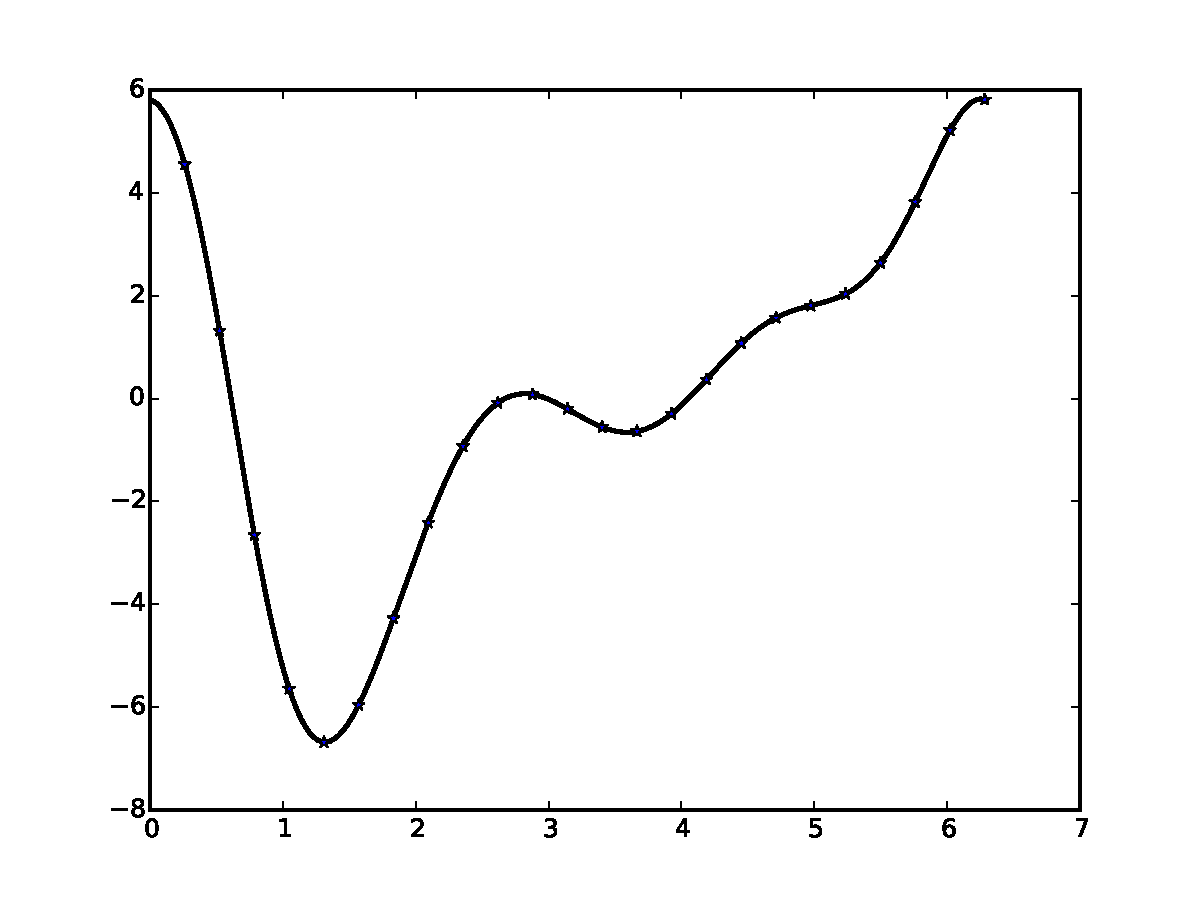
\includegraphics[width=\textwidth]{spectral2_derivative.pdf}
% \caption{The derivative of $u(x) = \sin^2 (x) \cos(x) +e^{2\sin(x+1)}$.}
% \label{fig:spectral:spectral2_derivative}
% \end{figure}
% 
% \begin{problem}
% Consider again the function $u(x) = \sin^2 (x) \cos(x) +e^{2\sin(x+1)}$.
% Create a function that approximates $\frac{1}{2}u''-u'$ on the Fourier grid points for a given $N$.	
% \end{problem}

% \begin{lstlisting}
% import numpy as np
% import matplotlib.pyplot as plt
% 
% # Solve the ODE $u_{xx} = e^u,$ with boundary conditions
% #  $u(0) = u(2\pi) = 0$
% 
% 
% \end{lstlisting}





% \section*{The advection equation}
% Recall that the advection equation is given by
% \begin{align}
% &{ }u_t + cu_x = 0
% \end{align}
% where $c$ is the speed of the wave (the wave travels to the right for $c > 0$).
% We will consider the solution of the advection equation on the circle; this essentially amounts to solving the advection equation on $[0,2\pi]$ and assuming periodic boundary conditions. 

% A common method for solving time-dependent PDEs is called the \textit{method of lines}. To apply the method of lines to our problem, we use our Fourier grid points in $[0,\pi]$: given an even $N$, let $h = 2\pi/N$, so that $\{x_1,\ldots,x_N\} = \{h,2h,\ldots,2\pi-h,2\pi\}$.  By using these grid points we obtain the collection of equations
% \begin{align}
% &{ }u_t(x_j,t) + cu_x(x_j,t) = 0, \quad t >0, \quad j = 1, \ldots N. \label{spectral2:method_oflines}
% \end{align}







% traveling wave solutions of a partial differential equation are solutions of the form $u(x,t) = u(x-st),$ where $s$ is the speed of the traveling wave.
% Thus a traveling wave solution is a solution that is a function of one variable, $\xi= x-st$.
% This new frame of reference corresponds to an observer moving along with the wave, so that the wave appears stationary as the observer studies it.

% \subsection*{Burgers' equation}
% We will examine the process of studying traveling wave solutions using Burgers' equation, a nonlinear PDE from gas dynamics.
% It is given by
% \begin{align}
% 	u_t + \left( \frac{u^2}{2} \right)_x = \nu u_{xx}, \label{eqn:Burgers_pde}
% \end{align}
% where $u$ and $\nu$ represent the velocity and viscosity of the gas, respectively.
% It models both the process of transport with the nonlinear advection term $(u^2/2)_x = u u_x$, as well as diffusion due to the viscosity of the gas ($\nu u_{xx}$).
% 
% Let us look for a traveling wave solution $u(x,t) = \hat{u}(x-st)$ for Burgers equation.
% We transform \eqref{eqn:Burgers_pde} into the moving frame $(x,t) \to (\bar{x},\bar{t}) = (x-st, t)$. In this frame \eqref{eqn:Burgers_pde} becomes
% \begin{align}
% 	u_{\bar{t}} - s u_{\bar{x}}+ \left(\frac{u^2}{2} \right)_{\bar{x}} = \nu u_{\bar{x}\bar{x}}
% 	\label{eqn:Burgers_pde_moving_frame}
% \end{align}
% % The coordinate system $(\bar{x},\bar{t})$ is called the moving frame because the traveling wave is stationary in this coordinate system.
% This new frame of reference corresponds to an observer moving along with the wave, so that the wave appears stationary as the observer studies it.
% Thus, $\hat{u}_{\bar{t}} = 0$, so that the wave profile $\hat{u}$ satisfies the ordinary differential equation
% \begin{align}
% 	 -s u_{\bar{x}}+ \left(\frac{u^2}{2} \right)_{\bar{x}} = \nu u_{\bar{x}\bar{x}}.
% 	\label{eqn:Burgers_ode}
% \end{align}
% 
% From here on we will drop the bar notation for simplicity.
% We seek a traveling wave solution with asymptotically constant boundary conditions; that is,  $\lim_{x \to \pm \infty}\hat{u}(x) = u_{\pm}$
% 
% both exist, and  $\lim_{x \to \pm \infty} \hat{u}'(x) = 0$.
% We will suppose that $u_- > u_+ > 0$.
% 
% % A traveling wave solution $u(\xi)$ of Burgers' equation will satisfy the ordinary differential equation
% % \[ -s u' + u u' = \nu u''.\]
% 
% Note that to this point we still don't know the speed of the traveling wave.
% Integrating both sides of this differential equation, and then taking the limit as $x \to +\infty$, we obtain
% \begin{align*}
% -s\int_{-\infty}^x u' + \int_{-\infty}^x \left(\frac{u^2}{2}\right)' &= \nu \int_{-\infty}^x u'',\\
% -s(u(x) - u_-) + \frac{u^2(x)}{2} - \frac{u_-^2}{2} &= \nu (u'(x) - u'(-\infty)), \\
% -s(u_+ - u_-) + \frac{u_+^2}{2} - \frac{u_-^2}{2} &= 0.
% \end{align*}
% Thus given boundary conditions $u_{\pm}$ at $\pm \infty$, the speed of the traveling wave must be $s = \frac{u_- + u_+}{2}$.
% 
% % Usually at this point, the traveling wave must be numerically solved using the profile ODE (\eqref{eqn:Burgers_ode} for Burgers equation).
% However, the profile ODE for Burgers is simple enough that it is possible to obtain an analytic solution.
% The traveling wave is  given by
% % If we continue by solving the first order equation
% % \[-\frac{u_- + u_+}{2}(u(x) - u_-) + \frac{u^2(x)}{2} - \frac{u_-^2}{2} = \nu u'(x)\]
% % we obtain a one-parameter family of solutions
% \[\hat{u}(x) = s - a \tanh \left(\frac{ax }{2\nu} + \delta\right)\]
% where $a = (u_- - u_+)/2$ and $\delta$ is fixed real number.
% We get a family of solutions because any translation of a traveling wave solution is also a traveling wave solution.
% 
% \subsection*{Stability of traveling waves}
% Suppose that an evolutionary PDE
% \begin{align}
% u_t = G(u,u_x, u_{xx}, \ldots).
% \label{eqn:evol_pde_repeat}
% \end{align}
% has a traveling wave solution $u(x,t) = \hat{u}(x-st)$.
% An interesting question to consider is whether the mathematical solution, $\hat{u}$, has a physical analogue.
% In other words, does the traveling wave show up in real life?
% This question is the start of the mathematical study of stability of traveling waves.
% 
% We begin by translating \eqref{eqn:evol_pde_repeat} into the moving frame $(x,t) \to (\bar{x},\bar{t}) = (x-st, t)$.
% In this frame the PDE becomes
% \begin{align*}
% u_t - su_x = G(u,u_x, u_{xx}, \ldots).
% \end{align*}
% In these coordinates the traveling wave is stationary.
% Thus, the solution of
% \begin{align*}
% \begin{split}
% u_t - su_x &= G(u,u_x, u_{xx}, \ldots), \\
% u(x,t = 0) &= \hat{u}(x),
% \end{split}
% \end{align*}
% is given by $u(x,t) = \hat{u}(x)$.
% We say that the traveling wave $\hat{u}$ is asymptotically orbitally stable if whenever $v(x)$ is a small perturbation of $\hat{u}(x)$, the general solution of
% \begin{align*}
% \begin{split}
% u_t - su_x &= G(u,u_x, u_{xx}, \ldots), \\
% u(x,t = 0) &= v(x),
% \end{split}
% \end{align*}
% converges to some translation of $\hat{u}$ as $t \to \infty$.
% Using this definition to prove stability of a traveling wave is a nontrivial task.
% 
% \subsection*{Visualizing stability of the traveling wave solution of Burgers' equation}
% The traveling wave solution of Burgers' equation is a stable wave.
% To view this numerically, we discretize the PDE
% \[u_t -su_x + uu_x = u_{xx}\]
% using the second order centered approximations
% % \begin{align*}
% % &{ } u_t(x_j,t_{n+1/2}) \approx \frac{u_j^{n+1}-u_j^n}{\triangle t}, \quad
% % u_x(x_j,t_{n+1/2}) \approx \frac{1}{2} \left( \frac{u_{j+1}^{n+1}-u_{j-1}^{n+1}}{2 \triangle x} +  \frac{u_{j+1}^{n}-u_{j-1}^{n}}{2 \triangle x}\right) ,\\
% % &{ } u_{xx}(x_j,t_{n+1/2}) \approx \frac{1}{2} \left( \frac{u_{j+1}^{n+1}- u_{j}^{n+1}+u_{j-1}^{n+1}}{(\triangle x)^2} + \frac{u_{j+1}^{n}- u_{j}^{n}+u_{j}^{n+1}}{(\triangle x)^2}\right).
% % \end{align*}
% \begin{align*}
% &{ } D_t U_j^{n+1/2} = \frac{U_j^{n+1}-U_j^n}{\triangle t}, \quad
% D_{xx}U_j^{n+1/2} = \frac{1}{2} \left( \frac{U_{j+1}^{n+1}-U_{j-1}^{n+1}}{2 \triangle x} +  \frac{U_{j+1}^{n}-U_{j-1}^{n}}{2 \triangle x}\right),\\
% &{ } D_{xx}U_j^{n+1/2} = \frac{1}{2} \left( \frac{U_{j+1}^{n+1}- U_{j}^{n+1}+U_{j-1}^{n+1}}{(\triangle x)^2} + \frac{U_{j+1}^{n}- U_{j}^{n}+U_{j-1}^{n}}{(\triangle x)^2}\right)
% \end{align*}
% 
% Substituting these expressions into the PDE we obtain a second-order, implicit Crank-Nicolson method
% % \begin{align*}
% % &{ }u_j^{n+1} + k_1 (u_j^{n+1}-s)(u_{j+1}^{n+1} - u_{j-1}^{n+1})
% % - k_2(u_{j+1}^{n+1} - 2u_j^{n+1}+ u_{j-1}^{n+1}) = \\
% % &{ } u_j^n - k_1(u_j^n-s) (u_{j+1}^n - u_{j-1}^n)
% % + k_2 (u_{j+1}^n -2u_j^n + u_{j-1}^n),
% % \end{align*}
% \begin{align*}
% U_j^{n+1} - U_j^n &= K_1 \big[(s - U_j^{n+1})(U_{j+1}^{n+1} - U_{j-1}^{n+1})
% + (s - U_j^n) (U_{j+1}^n - U_{j-1}^n) \big] \\
% &{ }  \quad
% + K_2 \big[(U_{j+1}^{n+1} - 2U_j^{n+1}+ U_{j-1}^{n+1}) + (U_{j+1}^n -2U_j^n + U_{j-1}^n) \big],\\
% &{ }  \quad
% \end{align*}
% where $K_1 = \frac{ \triangle t }{4 \triangle x}$ and $K_2 = \frac{ \triangle t}{2(\triangle x)^2}$.
% 
% \begin{problem}
% Numerically solve the initial value problem
% \begin{align*}
% 	&{ } u_t -su_x + uu_x = u_{xx}, \quad x \in (-\infty,\infty),\\
% 	&{ } u(x,0) = v(x),
% \end{align*}
% for $t \in [0,1]$.
% Let the perturbation $v(x)$ be given by
% \[v(x) = 3.5(\sin{(3x)} + 1)\frac{1}{\sqrt{2\pi}} \exp{(-x^2/2)}\]
% And let the initial condition be $u(x, 0) = \hat{u}(x) + v(x)$
% Approximate the $x$ domain,$(-\infty, \infty)$, numerically by the finite interval $[-20,20]$, and fix $u(-20) = u_-$, $u(20) = u_+$. Let $u_- = 5$, $u_+ = 1$.
% Use 150 intervals in space and 350 steps in time.
% Animate your results.
% You should see the solution converge to a translate of the traveling wave $\hat{u}$.
% 
% Hint: This difference scheme is no longer a linear equation.
% We have a nonlinear equation in $U^{n+1}$.
% We can still solve this function using Newton's method or some other similar solver.
% In this case, use \li{scipy.optimize.fsolve}.
% \end{problem}



% \section*{Traveling wave solutions of an evolution equation}
% Consider the transport equation together with initial conditions on the real line:
% \begin{align*}
% 	&{ }u_t + su_x  = 0, \quad -\infty < x < \infty, \\
% 	&{ }u(x,0) = f(x).
% \end{align*}
% This initial value problem has as its general solution the function $u(x,t) = f(x -st)$. Thus the function $f$ represents a 'signal' that is transported to the right with speed $s$.
% 
% In a similar fashion we may consider a general evolutionary PDE
% \begin{align}
% u_t = G(u,u_x, u_{xx}, \ldots),
% \label{lab:solitons:evol_pde}
% \end{align}
% and ask whether Equation \eqref{lab:solitons:evol_pde} has traveling wave solutions. 
% In other words, is there a signal or wave profile $f(x)$, so that $u(x,t) = f(x-st)$ is a solution of \eqref{evol_pde} that carries the signal at a constant speed $s$?
% 
% These traveling waves are often significant physically.  In a previous lab we looked at traveling 
% wave solutions of Burgers equation, an canonical equation in gas dynamics.  
% 
% 
% For example, in a PDE modelling insect population dynamics a traveling wave could represent a swarm of locusts; in a PDE describing a combustion process a traveling wave could represent an explosion or detonation.